\documentclass[a4paper,12pt]{article}
\usepackage{amsmath}
\usepackage{amsfonts}
\usepackage{amssymb}
\usepackage{hyperref}
\usepackage{subfig}
\renewcommand{\figurename}{Fig.}
\renewcommand*{\figureautorefname}{Fig.}
\usepackage{graphicx}

\graphicspath{[./images/]}
\usepackage{float}
\usepackage{multirow}
\usepackage{placeins}
\usepackage{color}
\usepackage{array}
\usepackage{cancel}
\usepackage[margin=1in]{geometry}
%\usepackage[left=1.5in, right=1.5in]{geometry}

\usepackage[nameinlink,noabbrev]{cleveref}
\crefname{equation}{eq.}{eqs.} % force abbreviated forms for equation "names"
\Crefname{equation}{Eq.}{Eqs.}
\crefname{figure}{fig.}{figs.}
\Crefname{Figure}{Fig.}{Figs.}


%\usepackage{cmbright}
%\renewcommand{\familydefault}{\sfdefault}

\newcommand{\diff}{\mathrm{d}}
\newcommand{\V}[1]{\boldsymbol{#1}}
\newcommand{\B}[1]{\mathbf{#1}}
\newcommand{\myhat}[2]{\hat{#1}_{#2}}
\renewcommand*\arraystretch{1.5}
\renewcommand{\div}[1]{\nabla_{#1} \cdot}
\newcommand{\lapl}{\nabla^2}
\newcommand{\grad}[1]{\nabla_{#1}}
\newcommand{\curl}{\nabla \times}
\newcommand{\Tr}{\mathrm{Tr}}
\newcommand{\op}[1]{\mathcal{#1}}

\newcommand{\yxb}[1]{  {\bf \color{red}{ Bao: #1}} }
\newcommand{\ygq}[1]{  {\bf \color{blue}{ Qin: #1}} }

\DeclareMathAlphabet\mathbfcal{OMS}{cmsy}{b}{n}


\title{Macroscopic Heat Transfer Model for Additive Manufacturing Testbed Problem}
\author{Yuanxun Bao and Yigong Qin}
\date{\today}


\begin{document}

\maketitle


\section{Macroscopic model}

We model the macroscopic heat transfer in the rectangular domain $\Omega$

\begin{equation}
\frac{\partial \rho c_{p} T}{ \partial t} = \div{} ( K \grad{} T) -\frac{\partial \rho L  f_l(T)}{\partial t} \quad \text{in }  \Omega
\end{equation}
\begin{equation}
\frac{\partial T}{ \partial t} = \alpha \Delta T - \frac{L}{c_p}\frac{\partial   f_l(T)}{\partial t} \quad \text{in }  \Omega
\end{equation}
with boundary conditions 
\begin{align}
(-K \grad{} T) \cdot \hat{n} = -q_s + h(T - T_e) + \epsilon \sigma (T^4 - T_e^4)  & \quad \text{on } \Gamma_{top} \\
(-K \grad{} T) \cdot \hat{n} = 0  & \quad \text{on } \Gamma  \backslash \Gamma_{top}
\end{align}
where $K$ is the heat conductivity, $\alpha$ is thermal diffusivity, $h$ is the convective heat transfer coefficient, $\epsilon$ is the thermal radiation coefficient, $\sigma$ is the Stefan-Boltzmann constant, and $L$ is the latent heat. The fluid mass fraction $f_l$ is modeled as
\begin{equation}
f_l(T) =
\left\{
\begin{array}{cc}
1 & T>T_l \\
\frac{T-T_s}{T_l - T_s} & T_s \leq T \leq T_l \\
0 & T < T_s
\end{array}
\right.
\end{equation}
where $T_l$ and $T_s$ are the liquidus and solidus temperature, respectively.
The heat source $q_S$ is modeled as a moving Gaussian
\begin{equation}
q_s(x, t ) = \frac{2Q\eta}{\pi r_b^2} \exp \left( -\frac{ 2(x-V_s t)^2}{ r_b^2} \right),
\end{equation}
where $Q$ is the source of heat power, $\eta$ is the absorption coefficient, $r_b$ is the radius of heat source and $V_s$ is the scanning speed.  

\section{Discretization}

We discretize the domain $\Omega$ using $(N+1) \times (M+1)$ grid with meshwidth $h$. Lx = Nh, x = ih.
Let $T_{ij}^n=T(ih, jh, t_n )$ for $i=0,\dots,N$ and $j = 0, \dots, M$.

\begin{equation}
\frac{T_{i,j}^n - T_{i,j}^{n-1}}{\Delta t} = \alpha \frac{T_{i,j+1}^n + T_{i,j-1}^n + T_{i-1,j}^n + T_{i+1,j}^n - 4 T_{i,j}^n }{h^2} - L_m \frac{\partial f_l(T) }{\partial t} \bigg|_{t = t_n}
\end{equation}
At the top boundary $(j=0)$, we treat the convection and radiation term explicitly,
\begin{equation}
-K \frac{T_{i, -1}^n - T_{i,1}^n}{2h} = -q_s (ih, t_n) + h (T^{n-1}_{i,0} - T_e) + \epsilon \sigma ( (T^{n-1}_{i,0})^4 - T_e^4), \ i = 0 , \dots , N
\end{equation}

\begin{equation}
T_{i, -1}^n = T_{i,1}^n -\frac{2h}{K}\left(-q_s (ih, t_n) + h (T^{n-1}_{i,0} - T_e) + \epsilon \sigma ( (T^{n-1}_{i,0})^4 - T_e^4)\right)=T_{i,1}^n+U_i^{n-1}, \ i = 0 , \dots , N
\end{equation}
Other boundaries:
\begin{align}
T_{i, M+1}^n =T_{i,M-1}^n, \ i = 0 , \dots , N\\
T_{-1, j}^n =T_{1,j}^n, \ j = 0 , \dots ,M\\
T_{N-1, j}^n =T_{N+1,j}^n, \ j = 0 , \dots ,M
\end{align}

Eventually, the linear system of equation should look like 
\begin{equation}
(\B{I} - C\B{L} ) \B{T}^n + \B{N} (\B{T}^n) = \B{T}^{n-1} +\B{N} (\B{T}^{n-1})+ \text{BC terms}
\end{equation}
where C is CFL number, $\B{L}$ is the discrete 2D laplacian with Neumann BCs and $\B{N}$ is a nonlinear function due the implicit treatment of latent heat term. If we treat the latent heat term explicitly, we need two starting values initially. 

\yxb{3. Can you find out what $\B{L}$, $\B{N}$ and BC terms are?}

\yxb{4. I am afraid we have to solve nonlinear system of equation due to the latent heat term.}

\section{Numerical Tests}

\subsection{No latent heat term}

\begin{equation}
\frac{T_{i,j}^n - T_{i,j}^{n-1}}{\Delta t} = \alpha \frac{T_{i,j+1}^n + T_{i,j-1}^n + T_{i-1,j}^n + T_{i+1,j}^n - 4 T_{i,j}^n }{h^2} 
\end{equation}

for top boundary (j=0)
\begin{equation}
\frac{T_{i,0}^n - T_{i,0}^{n-1}}{\Delta t} = \alpha \frac{T_{i,1}^n + T_{i,-1}^n + T_{i-1,0}^n + T_{i+1,0}^n - 4 T_{i,0}^n }{h^2} =\alpha \frac{2T_{i,1}^n + U_i^{n-1}+ T_{i-1,0}^n + T_{i+1,0}^n - 4 T_{i,0}^n }{h^2} 
\end{equation}
\begin{equation}
 \text{BC terms}=CU_i^{n-1},\ \  j=0,  \ i = 0 , \dots , N
\end{equation}
\begin{equation}
U_i^{n-1}=-\frac{2h}{K}\left(-q_s (ih, t_n) + h_c (T^{n-1}_{i,0} - T_e) + \epsilon \sigma ( (T^{n-1}_{i,0})^4 - T_e^4)\right), \ i = 0 , \dots , N
\end{equation}

\begin{equation}
q_s (ih, t_n) =q_0\exp \left( -\frac{ 2(ih-V_s t_n)^2}{ r_b^2} \right)= q_0\exp \left( -\frac{ 2(i-{V_s}^{'} t_n)^2}{{ r_b}^{'2}} \right) , \ i = 0 , \dots , N
\end{equation}
\\
\subsubsection{Test 1}
Parameters: K = 0.01, $\rho$ = 1.0, $C_p$ = 1.0, Q = 3, $\eta$ = 1, $r_b$ = 0.2, $V_s$ = 0.075. \\
Up boundary cooling parameters: $h_c$= 0.005, $\epsilon$ = 0.005, $\sigma$ = 5.67E-8, $T_e$ = 0.\\
Computation domain: $L_x$ = 8, $L_y$ = 2.



\begin{figure}[!ht]
     \subfloat[no surface cooling $h_c$= 0, $\epsilon$ = 0\label{subfig-1:nlatnrad}]{%
       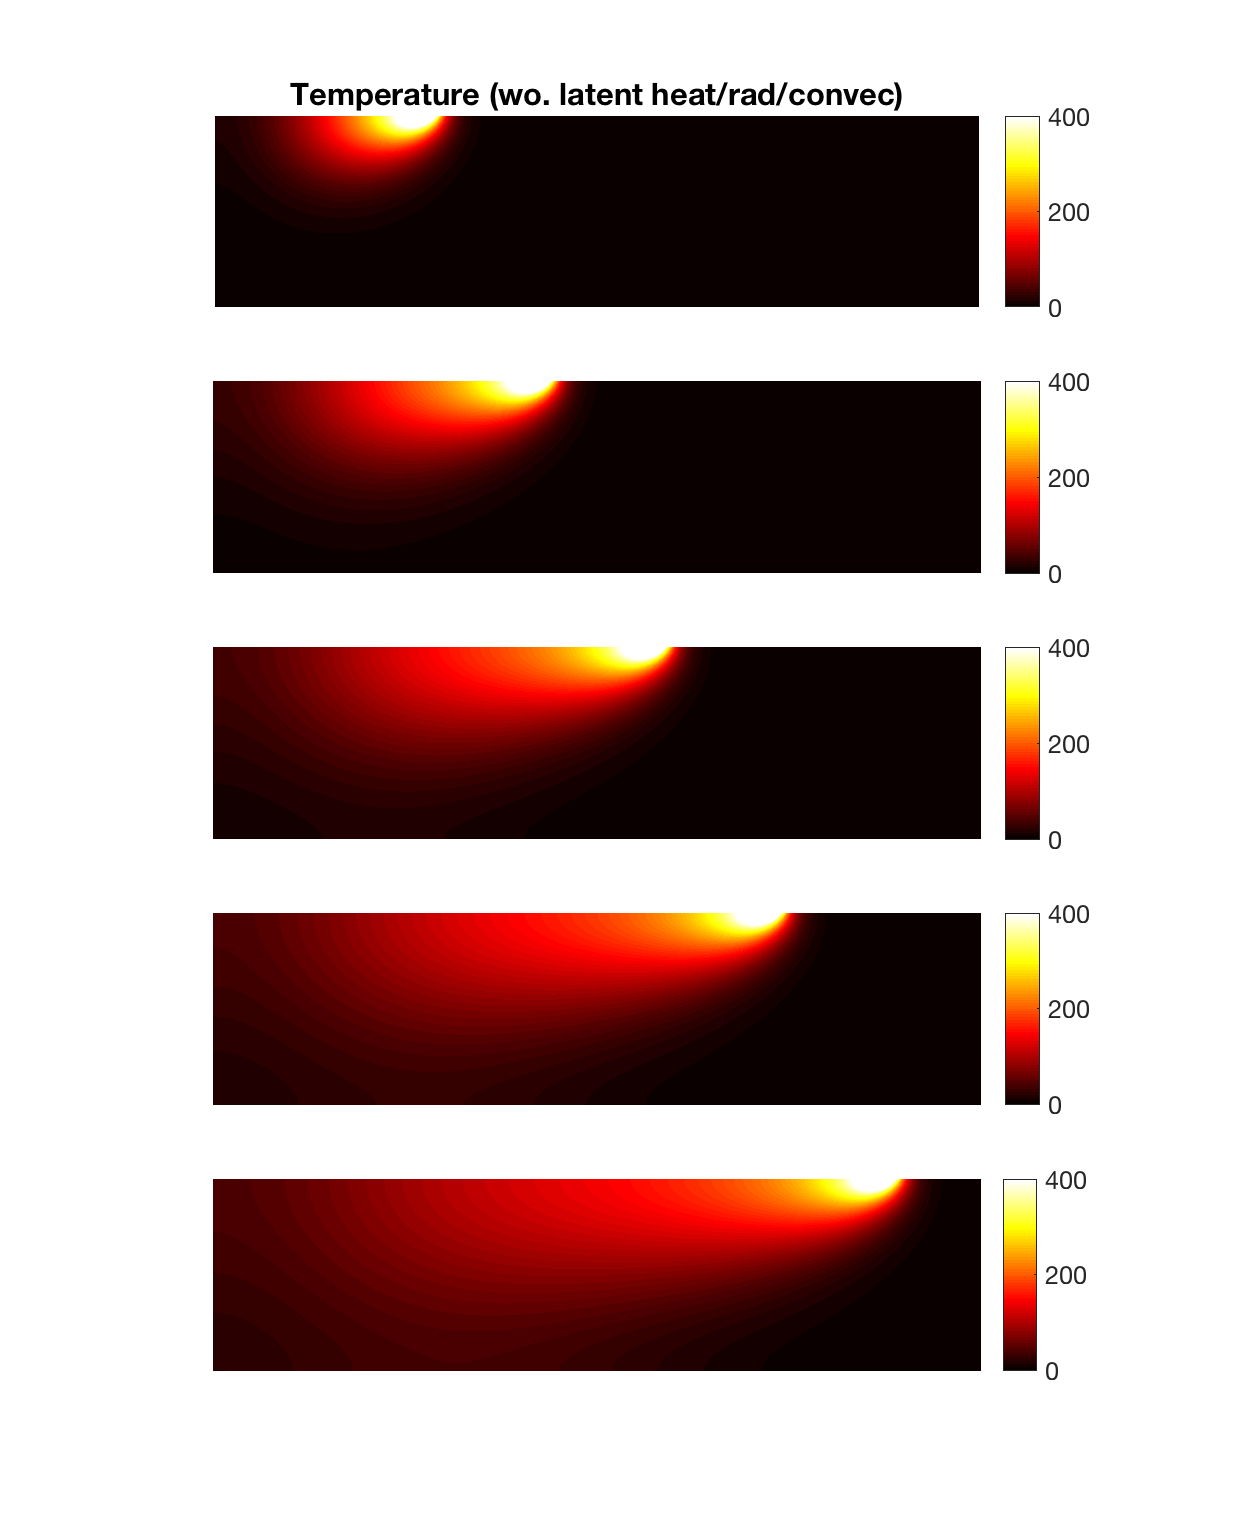
\includegraphics[width=0.45\textwidth]{./figures/temp_nlat_nrad.png}
     }
     \hfill
     \subfloat[$h_c$= 0.005, $\epsilon$ = 0.005\label{subfig-2:nlatwrad}]{%
       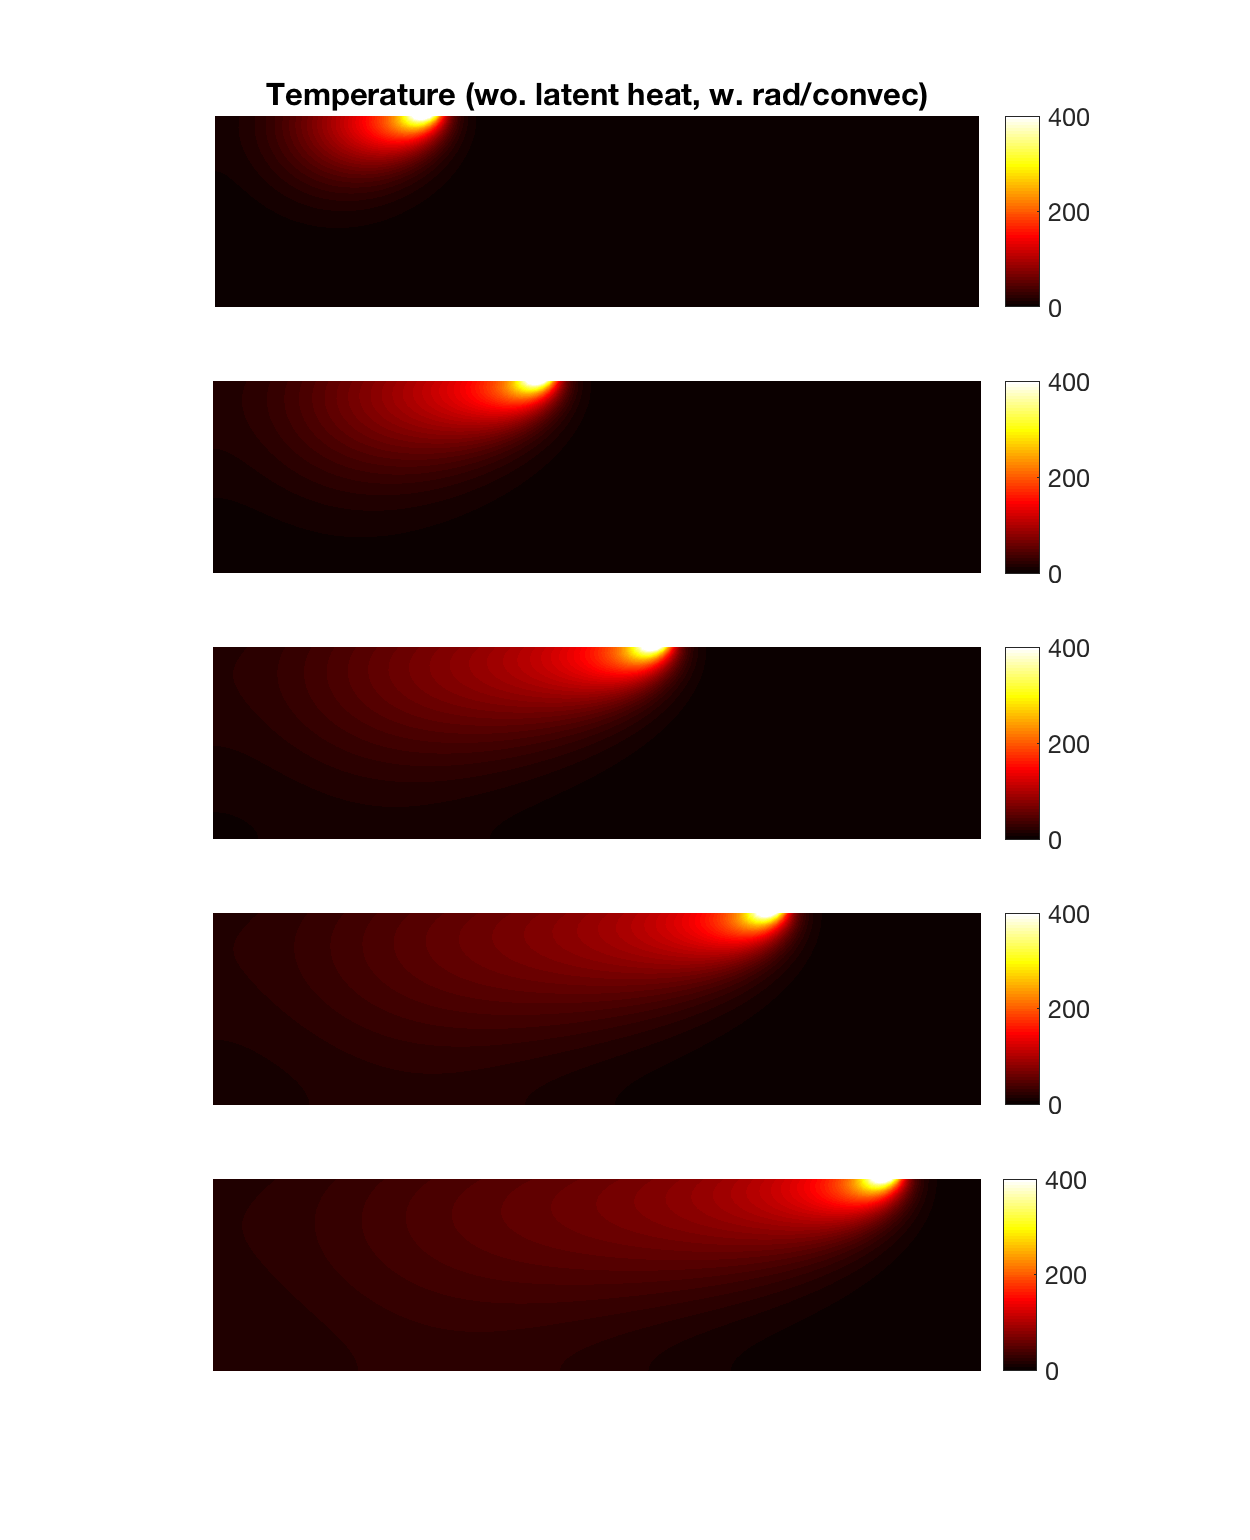
\includegraphics[width=0.45\textwidth]{./figures/temp_nlat_wrad.png}
     }
     \caption{Temperature distribution without latent heat.}
     \label{fig:nolatent}
   \end{figure}

\subsubsection{Self Convergence Study (with convection and radiation)}

Ground truth: dt = 0.00625, h = $ L_x/2048 $\\
Trial: dt = 0.025, 0.1, 0.4, 1.6; h =  $ L_x/1024, L_x/512, L_x/256, L_x/128 $

\begin{figure}[!ht]
     \subfloat[$L^2$ error \label{subfig-1:dummy}]{%
       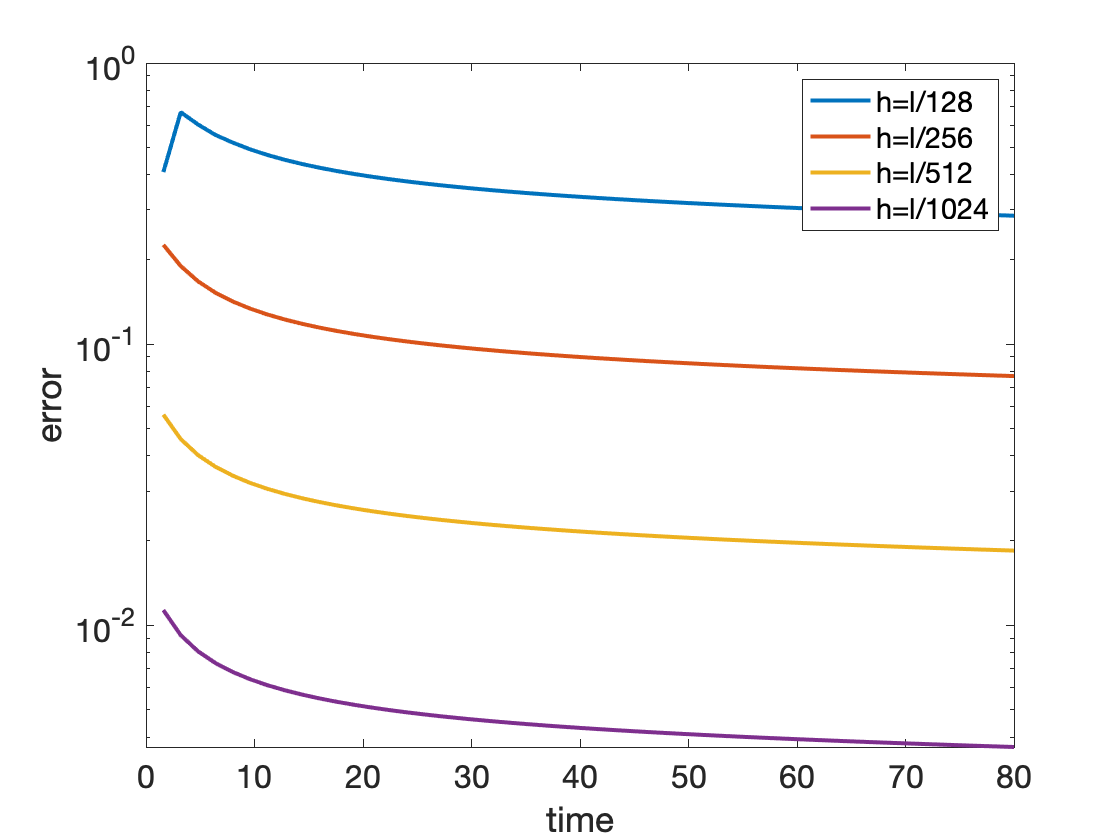
\includegraphics[width=0.45\textwidth]{./figures/self_convergence.png}
     }
     \hfill
     \subfloat[convergence order 2.076\label{subfig-2:dummy}]{%
       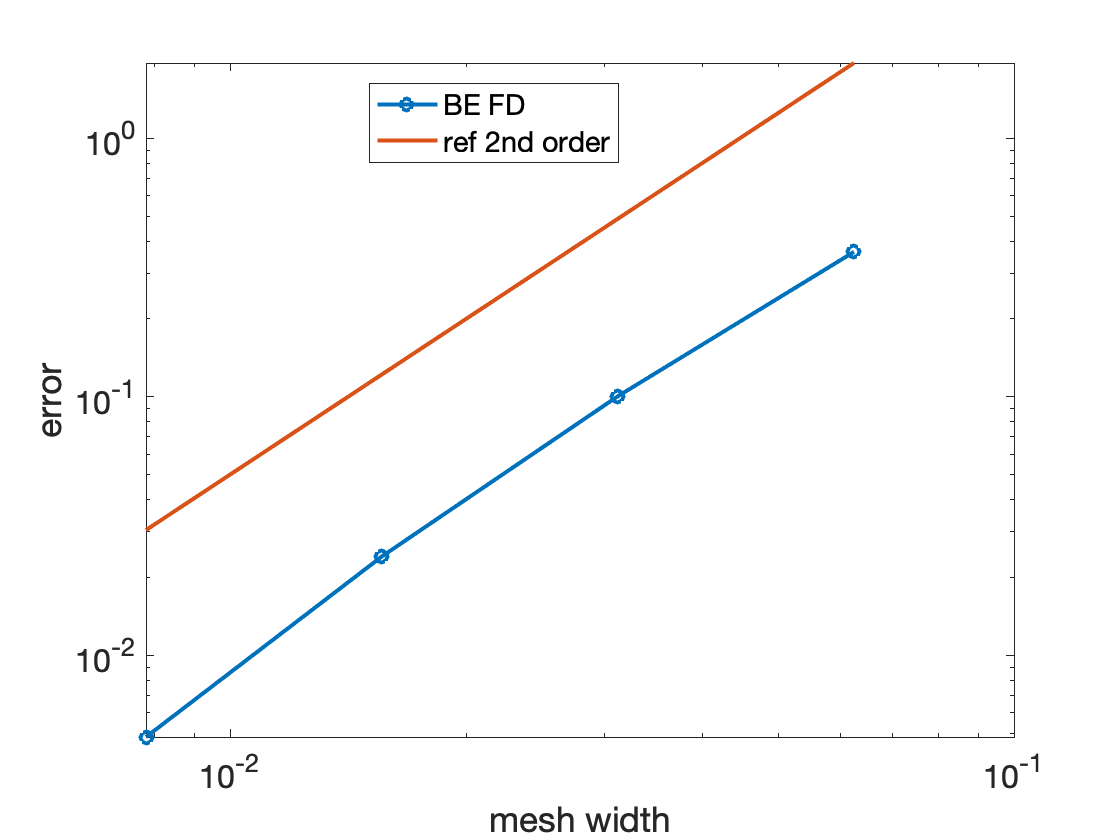
\includegraphics[width=0.45\textwidth]{./figures/Convergence_order.png}
     }
     \caption{Self convergence. }
     \label{fig:nolat_convergence}
   \end{figure}


\subsection{Latent heat term implicit-explicit}
Implicit: 
\begin{equation}
\frac{\partial   f_l(T)}{\partial t} = \frac{f_l^{n}(T)-f_l^{n-1}(T)}{\Delta t} 
\end{equation}
Explicit: 
\begin{equation}
f_l^{n}(T) =
\left\{
\begin{array}{cc}
1 & T^{n-1}>T_l \\
\frac{T^n-T_s}{T_l - T_s} & T_s \leq T^{n-1} \leq T_l \\
0 & T^{n-1} < T_s
\end{array}
\right.
\end{equation}

\begin{equation}
f_l^{n-1}(T) =
\left\{
\begin{array}{cc}
1 & T^{n-1}>T_l \\
\frac{T^{n-1}-T_s}{T_l - T_s} & T_s \leq T^{n-1} \leq T_l \\
0 & T^{n-1} < T_s
\end{array}
\right.
\end{equation}


\begin{equation}
\text{Latent heat term}=
\left\{
\begin{array}{cc}
0 & T^{n-1}>T_l \\
-\frac{L_m}{\Delta t}\frac{T^{n}-T^{n-1}}{T_l - T_s} & T_s \leq T^{n-1} \leq T_l \\
0 & T^{n-1} < T_s
\end{array}
\right.
\end{equation}
\\
\subsubsection{Test2}
Parameters: $L$=200, $T_s$=40, $T_l$=110\\

\begin{figure}[!ht]
     \subfloat[Without latent heat\label{subfig-1:nlat}]{%
       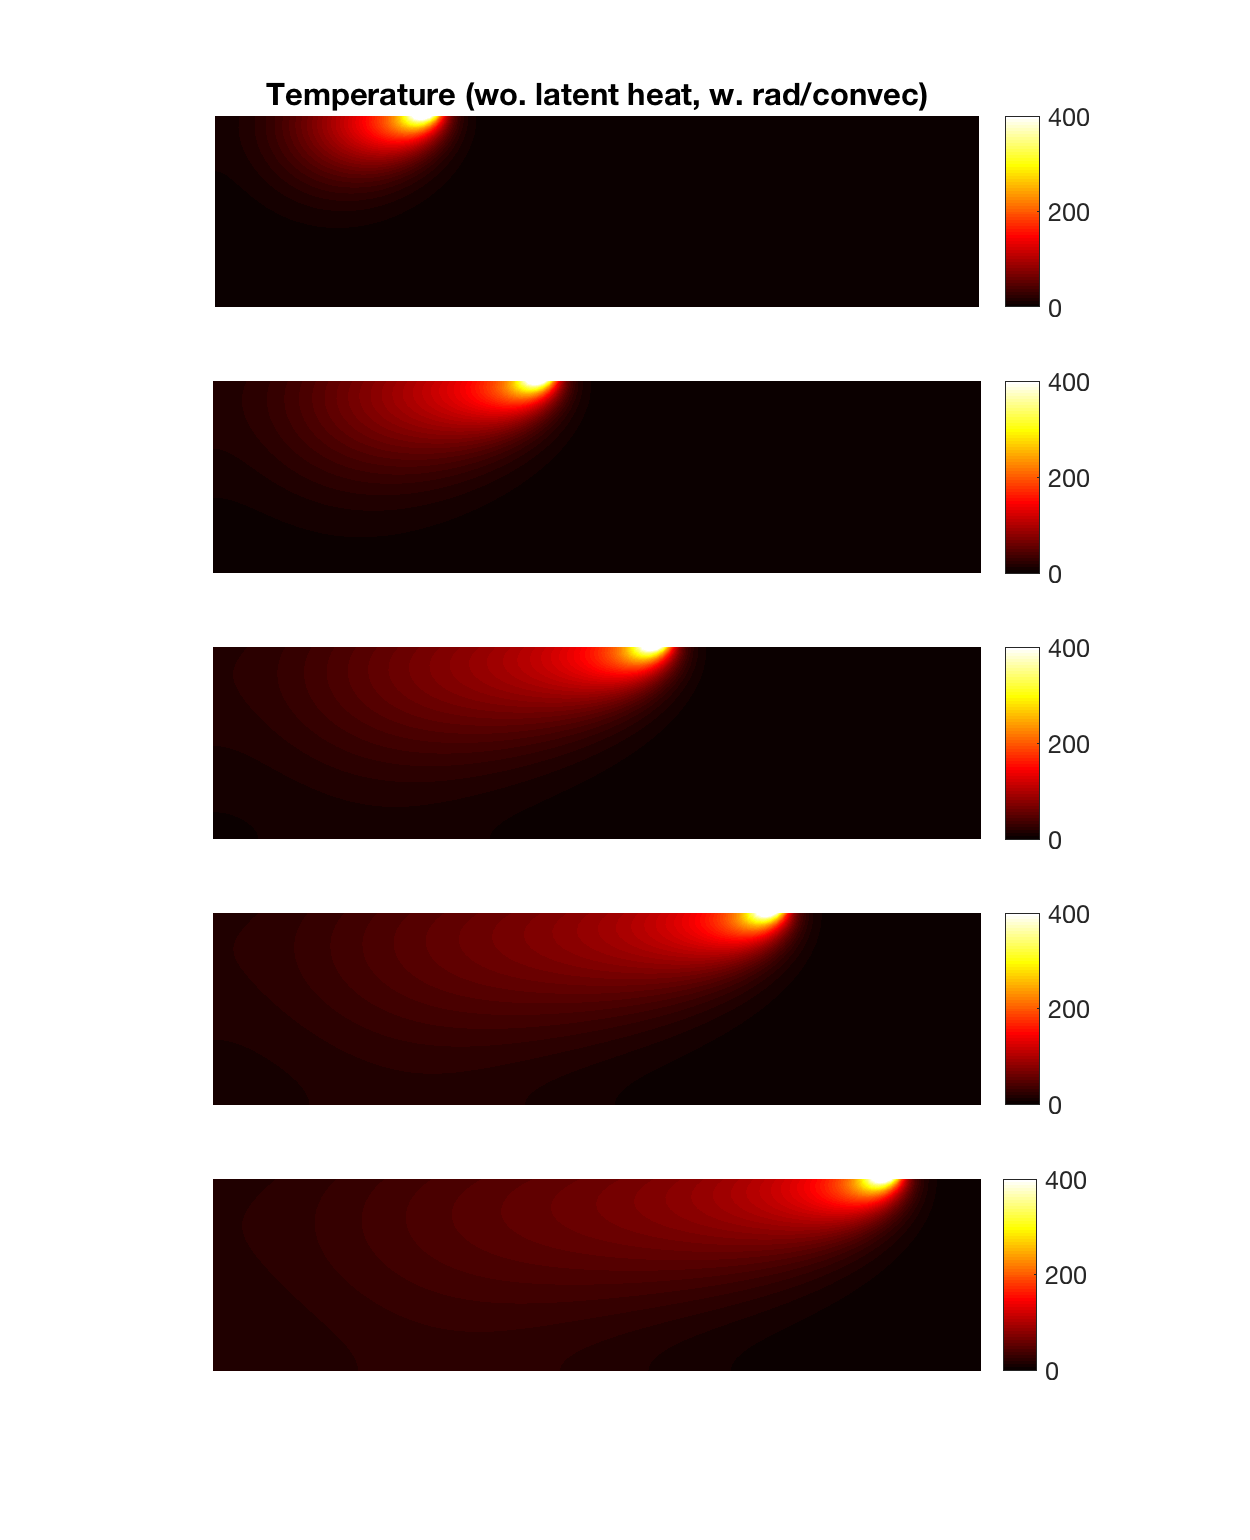
\includegraphics[width=0.45\textwidth]{./figures/temp_nlat_wrad.png}
     }
     \hfill
     \subfloat[With latent heat \label{subfig-2:lat}]{%
       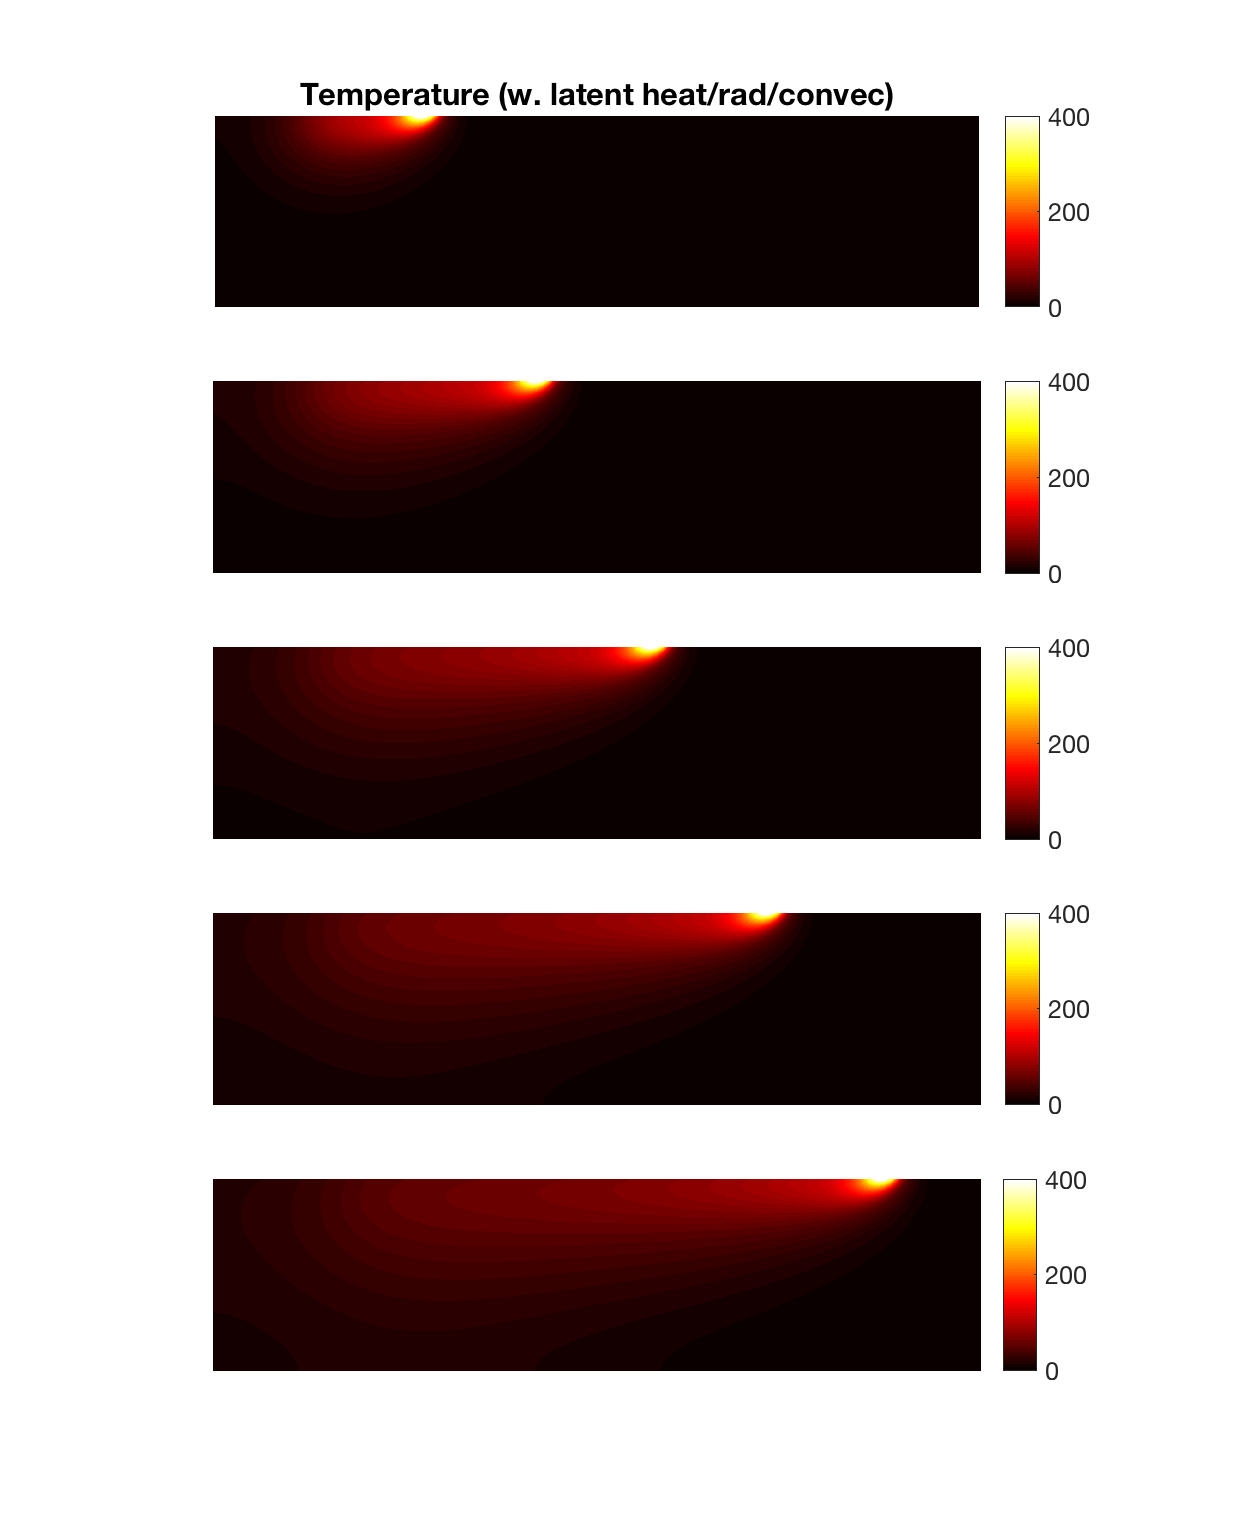
\includegraphics[width=0.45\textwidth]{./figures/temp_wlat_wrad.png}
     }
     \caption{Temperature distribution with and without latent heat. Surface cooling is included.}
     \label{fig:temp}
   \end{figure}


\begin{figure}[!ht]
     \subfloat[$L^2$ error \label{subfig-1:dummy}]{%
       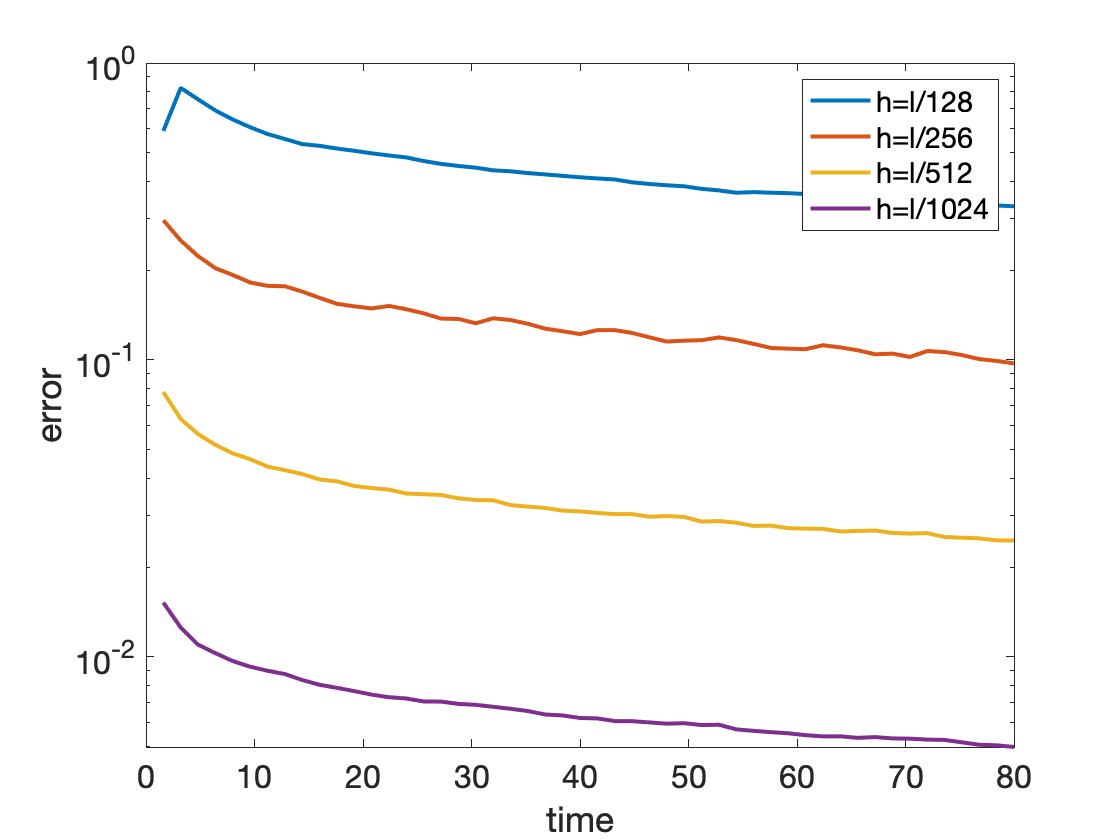
\includegraphics[width=0.45\textwidth]{self_lat.png}
     }
     \hfill
     \subfloat[convergence order\label{subfig-2:dummy}]{%
       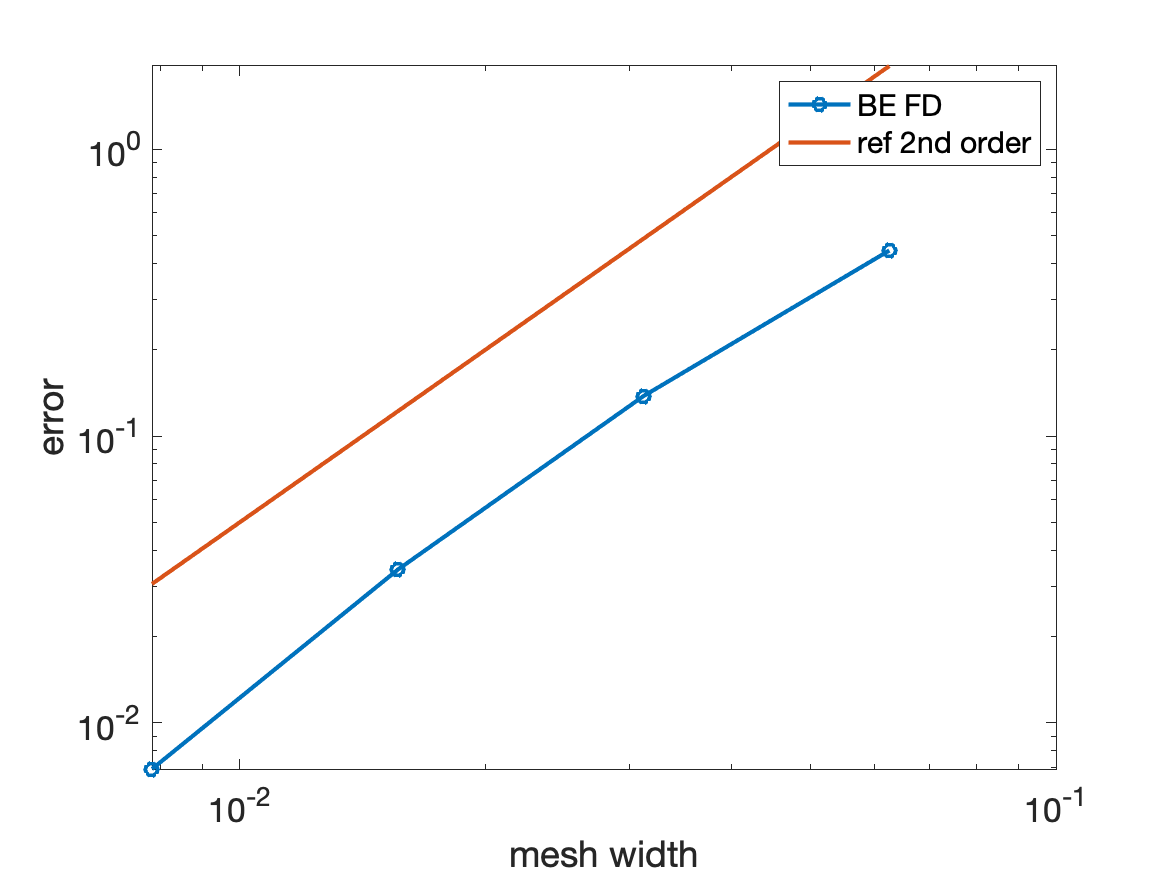
\includegraphics[width=0.45\textwidth]{convergence_lat.png}
     }
     \caption{Self convergence. }
     \label{fig:nolat_convergence}
   \end{figure}
GMRES solver (Tol = 1e-9):\\
For mesh width h =  $ L_x/1024, L_x/512, L_x/256, L_x/128 $\\
Iterations per time step without precondtioner: 58, 54, 48, 49, 50\\
Iterations per time step with precondtioner: 20, 17, 16,...      \ \        but took longer time to run


% \bibliographystyle{unsrt}
% \bibliography{../library.bib}



%%%%%%%%%%%%%%%%%%%%%%%%%%%%%%%%%%%%%%%%%%%%%%%

\end{document}
